\documentclass[twocolumn]{aastex63}

\usepackage{natbib}

\usepackage{graphicx}
\usepackage{epstopdf}
\usepackage{amsmath}
\usepackage{amssymb}
\usepackage{bm}
\usepackage{color}
\usepackage{multirow}
\usepackage{rotating}
\usepackage{makecell}



%%%%%%%%%%%%%BEGIN PAPER %%%%%%%%%%%%%%%%%%%%%%%%%%%%%

%\shorttitle{} 
 
\begin{document}

\title{Home court advantage in the COVID-19 pandemic, and machine learning March Madness}

\author[0000-0002-4645-6578]{Peter R. Williams}

%%%%%%%%%%%%%%%%%%%%%%%%%%%%%%%%%%%%%%
%%%%%%%%%%%%%%%%%%%%%%%%%%%%%%%%%%%%%%
%%%%%%%%%%%%%%%%%%%%%%%%%%%%%%%%%%%%%%
%%%%%%%%%%%%%%%%%%%%%%%%%%%%%%%%%%%%%%

\section{Motivation}
\label{sect:intro}
Home court advantage or home field advantage is a well documented phenomenon in sports in which the team playing on their home turf has a slight statistical edge over their opponent.
There are many factors that could be the source of the advantage:
\begin{itemize}
\item Familiarity with the court or field's intricacies, more likely to be a factor in baseball in which each field's dimensions are different
\item Familiarity with the home environment, such as weather or altitude
\item Psychological effect of favorable fans on the players
\item Psychological effect of fans on the referees or umpires
\item Physical toll of travel to away games
\end{itemize}

Every year, Kaggle hosts a ``Machine Learning Mania'' competition in which participants can submit machine learning models to predict the results of the NCAA basketball tournament, March Madness.
The competition comes with a rich data set with game results dating back to the 1984-85 season and more detailed game-by-game box scores since the 2002-03 season.
Many of the recent games even have play-by-play information, including where on the court and at what time shots and passes were made.

This year, I decided to use the data set to explore two things: 1) Examine how the lack of fans during the COVID-19-affected 2020-21 and 2021-22 seasons influenced home court advantage, and (of course) 2) write a machine learning algorithm to predict my March Madness bracket and win free dinner and beer from my friends.

\section{Home court advantage}
\label{sect:homecourt}

I can quantify the home court advantage by looking at the distribution of score differentials in a season. 
I'll define the score differential as 
\begin{multline}
{\rm Score~differential} = {\rm Score~of~home~team}\\
 - {\rm Score~of~away~team}.
\end{multline}
I'll then define the home court advantage as the mean value of the score differentials.
If, on average, home teams score 2 more points than away teams, the home court advantage would be 2 points.

\subsection{COVID-19 seasons}

One major difference between the 2020-21 and 2021-22 seasons compared to other seasons is that most schools opted to only play in-conference games.
This eliminated ``money games'' in which smaller schools would travel to play big-name schools and get a hefty pay check in return.
Money games often result in an easy, lopsided victory for the bigger school, and would therefore skew the distribution of score differentials. 
Because of this, I'll only look at in-conference games for every season.

The left panel of Figure \ref{fig:score_diff} shows Gaussian KDE fits to the score differential distributions for the 2015-16 to 2021-22 seasons, and the right panel shows a zoomed-in version.
The home court advantages are shown by the vertical dashed lines with their standard errors shown above.
All values dating back to the 1984-85 season are listed in Table \ref{tab:homecourtadvange}.
The 2020-21 and 2021-22 season home court advantages are less than those of every other season by an amount greater than the standard error, with the exception of the 2016-17 season.

\begin{figure*}
\centering
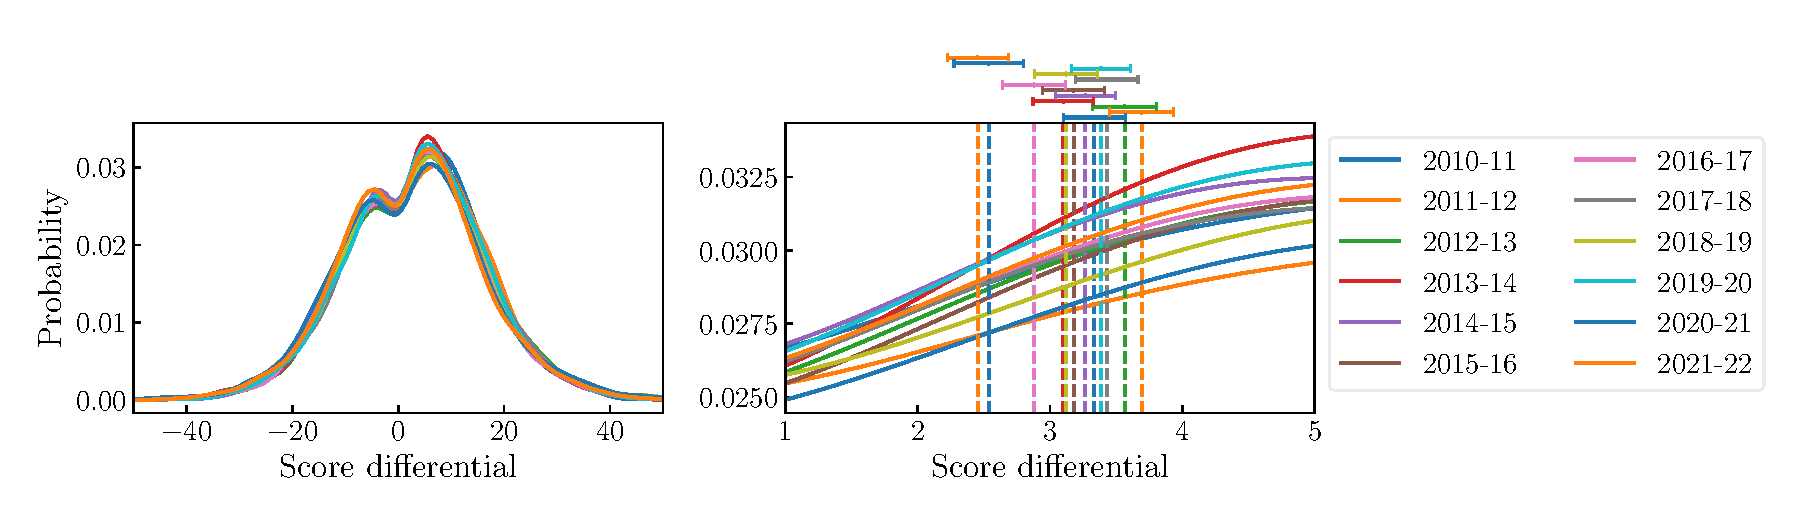
\includegraphics[width=7.2in]{figs/score_differential.pdf}
\caption{\textit{Left}: Score differentials for the 2010-11 to 2021-22 seasons. Note that the dip at 0 exists because ties aren't allowed. \textit{Rght}: Zoom-in of the left-hand panel with the home court advantage shown by the vertical dashed lines. Above the dashed lines, we show the standard error.}
\label{fig:score_diff}
\end{figure*}

\begin{deluxetable*}{lc|lc|lc|lc|lc}
\tabletypesize{\small}
\tablecaption{Home court advantage}
\tablewidth{0pt}
\tablehead{ 
\colhead{Year} &
\colhead{Advantage} &
\colhead{Year} &
\colhead{Advantage} &
\colhead{Year} &
\colhead{Advantage} &
\colhead{Year} &
\colhead{Advantage} &
\colhead{Year} &
\colhead{Advantage}
}
\startdata
1984-85 & $3.86 \pm 0.26$ & 1992-93 & $4.12 \pm 0.27$ & 2000-01 & $4.34 \pm 0.25$ & 2008-09 & $3.42 \pm 0.24$ & 2016-17 & $2.88 \pm 0.24$ \\
1985-86 & $3.90 \pm 0.26$ & 1993-94 & $3.98 \pm 0.27$ & 2001-02 & $4.29 \pm 0.25$ & 2009-10 & $3.45 \pm 0.23$ & 2017-18 & $3.43 \pm 0.24$ \\
1986-87 & $3.92 \pm 0.28$ & 1994-95 & $3.64 \pm 0.27$ & 2002-03 & $4.02 \pm 0.25$ & 2010-11 & $3.33 \pm 0.23$ & 2018-19 & $3.12 \pm 0.24$ \\
1987-88 & $4.63 \pm 0.28$ & 1995-96 & $3.67 \pm 0.27$ & 2003-04 & $3.87 \pm 0.25$ & 2011-12 & $3.69 \pm 0.24$ & 2019-20 & $3.38 \pm 0.22$ \\
1988-89 & $4.27 \pm 0.29$ & 1996-97 & $4.36 \pm 0.26$ & 2004-05 & $3.77 \pm 0.24$ & 2012-13 & $3.56 \pm 0.24$ & 2020-21 & $2.54 \pm 0.26$ \\
1989-90 & $4.42 \pm 0.28$ & 1997-98 & $3.93 \pm 0.28$ & 2005-06 & $3.59 \pm 0.24$ & 2013-14 & $3.10 \pm 0.23$ & 2021-22 & $2.45 \pm 0.23$ \\
1990-91 & $4.04 \pm 0.29$ & 1998-99 & $4.13 \pm 0.27$ & 2006-07 & $3.83 \pm 0.24$ & 2014-15 & $3.27 \pm 0.23$ &  & \\
1991-92 & $4.24 \pm 0.29$ & 1999-00 & $4.10 \pm 0.27$ & 2007-08 & $4.00 \pm 0.24$ & 2015-16 & $3.18 \pm 0.23$ &  &
\enddata
\tablecomments{Home court advantage (in points) and standard error for every season from 1984-85 to 2021-22. 
\label{tab:homecourtadvange}}
\end{deluxetable*} 

To further quantify the significance of the home court advantage decrease, I perform two-sample Kolmogorov-Smirnov (KS) tests using the score differential distributions.
The KS test is a statistical test used to indicate the probability that two samples are drawn from the same underlying distribution.
I perform the test for every combination of seasons from the 2009-10 to 2021-22 seasons, and show the $p$-values in Figure \ref{fig:kstest} (where the null hypothesis is that the score differentials are all drawn from the same distribution).
The values for the pairs involving the 2020-21 and 2021-22 seasons are given in Table \ref{tab:kstest}.
The 2020-21 and 2021-22 seasons are different from almost every other season (excluding each other) with $p$-value $<0.1$.
Notable exceptions are, again, the 2016-17 season with $p\sim0.3$ and the 2018-19 seasons with $p\sim 0.11$.


\begin{figure}
\centering
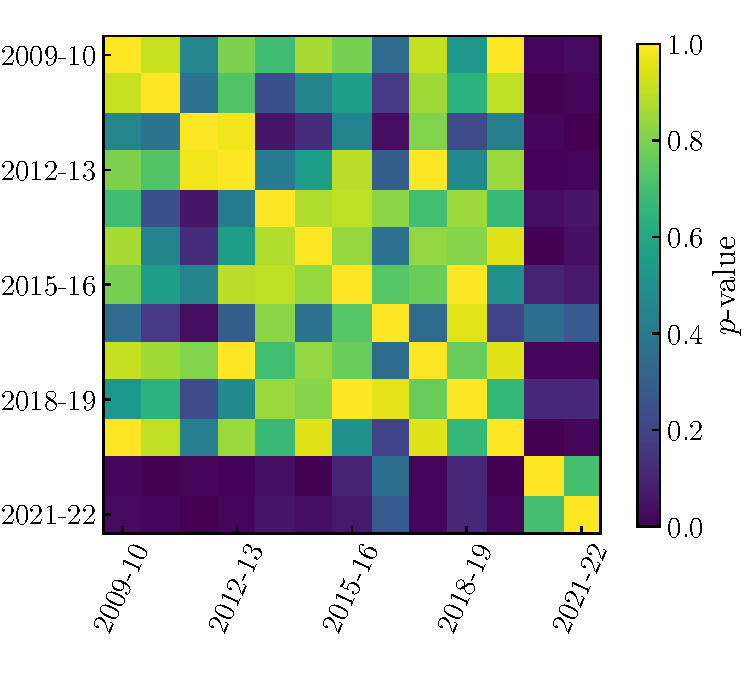
\includegraphics[width=3in]{figs/kstest.pdf}
\caption{$p$-values from the KS tests comparing all seasons dating back to the 2009-10 season. Note that 1) the bottom-left and top-right halves of the figure are mirror images of each other, and 2) the diagonal is unity since the two samples (from the same year) are identical.}
\label{fig:kstest}
\end{figure}

\begin{deluxetable}{l|cc}
\tabletypesize{\small}
\tablecaption{KS Test $p$-values}
\tablewidth{0pt}
\tablehead{ 
\colhead{} &
\colhead{2020-21} &
\colhead{2021-22}
}
\startdata
2009-10 & 0.012 & 0.029 \\
2010-11 & 0.004 & 0.012 \\
2011-12 & 0.012 & 0.001 \\
2012-13 & 0.011 & 0.013 \\
2013-14 & 0.038 & 0.060 \\
2014-15 & 0.006 & 0.041 \\
2015-16 & 0.096 & 0.068 \\
2016-17 & 0.362 & 0.285 \\
2017-18 & 0.013 & 0.014 \\
2018-19 & 0.115 & 0.110 \\
2019-20 & 0.002 & 0.015 \\
2020-21 & 1.000 & 0.704 \\
2021-22 & 0.704 & 1.000
\enddata
\tablecomments{KS test $p$-values comparing the score differential distributions for the 2020-21 and 2021-22 seasons vs. other seasons. 
\label{tab:kstest}}
\end{deluxetable} 

While the decrease in home court advantage may seem small (only 0.5-1 point), it is not at all insignificant.
One point can be the difference between ending the game in a loss versus taking it into over time. 
From the 2009-10 to 2019-20 seasons, the home team won 60.6\% of all games.
For the 2020-21 and 2021-22 seasons, that value dropped to 57.7\% and 57.9\%, respectively.
This alone accounts for 80 and 87 games, respectively, going to the away team rather than the home team.

These results demonstrate the importance of a strong fan-base that shows up to support its team, as the fans were the primary change from the COVID-19-affected seasons and the others.
Factors such as home court familiarity and travel likely still play a role in a team's success, but they are factors that remained unchanged in this analysis.
It isn't clear based on this analysis whether it's the players or the referees that are affected more by the fans: Do players play better when they're being cheered for, or do referees feel pressured to make certain calls when the whole arena is shouting at them?
Analyses of soccer games played during the pandemic found that referees give more yellow cards to home yeams than when the stadium is full.
A similar analysis could be done to disentangle the two effects by, e.g., looking at fouls handed out by refs or by looking at player stats such as field goal percentage and turnovers.

\subsection{Change over time and conference comparisons}
It is also interesting to explore how home court advantage has changed over time. 
Some factors that might cause a change are:
\begin{itemize}
\item Increased athletic department spending leading to improved accommodations and less travel fatigue
\item Changes in fan willingness to travel to away games
\item Conferences expanding, leading to further travel to away games
\item Changes in referee behavior as the camera puts them under scrutiny
\end{itemize}
In Figure \ref{fig:homecourtadvantage_vs_year}, I show the 5 year moving average of the home court advantage for some of the major basketball conferences.
Additionally, I've grouped the ``Power 5'' (AAC, Big 10, Big 12, Pac 12, and SEC) and ``Group of 5'' (AAC, C-USA, MAC, MW, Sun Belt) conferences together.
While these classifications are typically used in the context of college football, they're roughly correlated with the size and funding of the whole athletic departments.
I also show the Ivy League, which has notoriously low attendance at its games.
Perhaps unsurprisingly, the Ivy League has the lowest home court advantage compared to the powerhouse conferences, which may be due to the effect fans have as discussed above.

There is an overall decreasing trend to home court advantage, at least averaged over the Power 5 and Group of 5 conferences.
Interestingly, the decrease for both begins around the same time---the early 2000s.
This is before some of the major conference realignments of the 2010s such as the Big 10 expanision in the early 2010s, Pac 10 to Pac 12 expansion in 2010, SEC expansion in 2012, or Big East re-founding in 2013, so that is unlikely to be a contributing factor.
For the 2008-09 season, the three point arc was extended, but this would affect both the home and away teams similarly.
One possible culprit is the increased adoption of instant replay in the early 2000s.
As fans began to see important plays up close, the referees were put under increased pressure to make the right call, regardless of the pressure (whether conscious or unconscious) from the fans in the arena.
Now that teams are allowed to challenge calls in the NCAA, it will be interesting to see if the trend continues.

\begin{figure*}
\centering
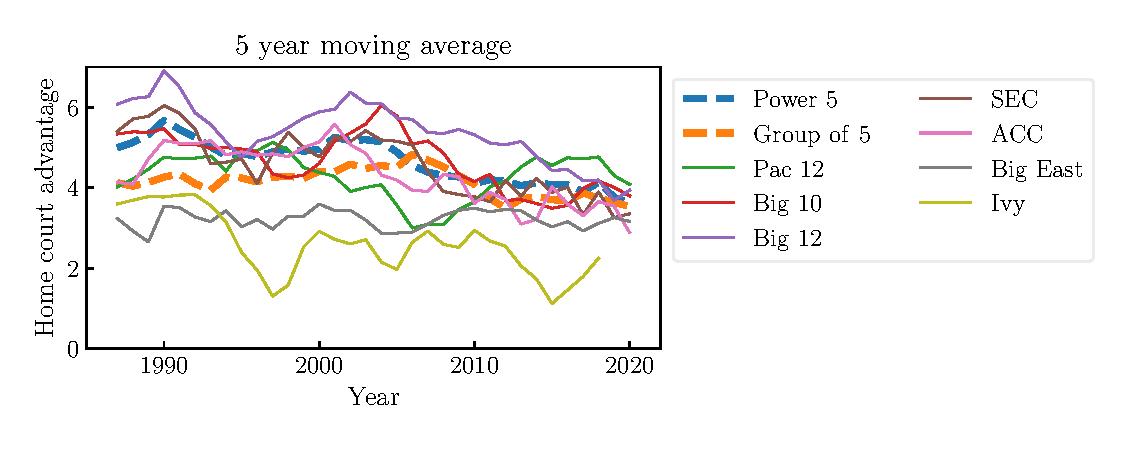
\includegraphics[width=6in]{figs/homecourtadvantage_vs_year.pdf}
\caption{Home court advantage over time for some of the major conferences and conference groups. A more detailed, interactive version is available at \textcolor{red}{LINK TO ONLINE VERSION}}
\label{fig:homecourtadvantage_vs_year}
\end{figure*}

\section{March Madness bracket}
\label{sect:marchmadness}
The above has all been fun, but it's pretty useless for the rest to come.
March Madness is played on neutral courts, so I can't use anything I've learned about home court advantage to make tournament predictions.
It might be possible to come up with some other metrics such as, ``how far did each team have to travel?''; ``do the team's fans travel well?''; ``how similar is the playoff location to the team's home location?''
If these factors are correlated with score differential, I could use a ``close-to-home-court'' advantage, but that's a project for the 2023 tournament.
Instead, I'll stick with the data that are easily accessible via the Kaggle-provided files.

\subsection{What exactly am I doing?}
The basic idea of the machine learning bracket predictions is that you can look at ``features'' such as team rankings, free throw percentage, turnovers, etc., and use those to predict which team will win each round based on data from the regular season and past regular season and tournament games.
Selecting which features to use is the first major decision-making step---a comparison between two teams' field goal percentages is \textit{much} more likely to predict which team will win than a comparison of which colors the teams are wearing (although always picking the blue team might not be a bad strategy...).
Once you've chosen your features, you can work with various machine learning algorithms that will try to figure out how to utilize the features to predict which teams will win.
Again, a bad model might say ``always pick the home team,'' but a better model will utilize all other information but give the home team a tiny boost.

The downside (or benefit, depending on how you want to look at it) of machine learning models is that you don't always know \textit{why} the model is making the decisions it's making, you usually just get to see the outcome.
This can be nice since 1) you don't need to be involved in every step of the decision making process and 2) the algorithm might find patterns that a human would miss.
The downside is that you might think the algorithm is doing a great job based on the training results when in fact the reasons it's making its decisions are very specific to the training set and are actually complete bogus.
Take, for instance, the early days of self driving cars that trained themselves to keep sidewalks and buildings on the side, and then freaked out when they needed to cross a bridge.

Because of this, it's standard practice to set aside some fraction of your data to validate on. 
Since the final goal of this project is to predict the results of the 2022 playoff games, it might make the most sense to train and validate the models using only playoff games.
However, the data set of playoff games is too small to adequately train a model.
Instead, I'll use all games (regular season + tournament) from the 2014-15 season onward for training.
I will, however, use only the playoff games for the validating set.
Due to time limits and computational resources, I'm only using the 2014-15 seasons onward and not using data from previous seasons.
Gameplay has changed since 1985, though, so this might not be a downside.

Finally, the quantity that I will train the models to predict will not be ``win'' or ``lose,'' but rather the score differential.
A 20 point blowout is more significant than a buzzer beater win, and the score differential contains that information.
For this, I'll use regressor models rather than classifiers.
When selecting my final bracket, it is straightforward to pick the winner based on the score differential.

\subsection{Feature and model selection}
Since I want to determine the probability that Team A beats Team B, it is useful to look at the difference in statistics between the two teams.
For instance, if Team A is ranked \#1 in the nation and Team B is ranked \#10, they're both very likely to win games \textit{in general}, but the more useful statistic is ``Team A is ranked 9 spots higher than Team B.'' 
For this reason, the features I will feed into the model will all be the difference in statistics between the two teams.

I'll start by considering some obvious ones:
\begin{itemize}
\item Team rankings: People get paid the big bucks to come up with these rankings, I might as well use their hard work for my benefit. There are 45 different ranking systems available in the Kaggle data set, so I'll pick just one or two. Since rankings change over the course of the season, I'll use the rankings as they are at the start of the tournament. This is based on the assumption that teams' abilities don't change significantly over the course of the season. Rather, the ability of rankers to accurately rank teams improves as more data come in.
\item Team seeds: Again, someone already put in the work to seed the bracket. I'll use it.
\item Win percentage: Teams that win a lot are probably good at winning. Unless...
\item Strength of schedule: ...unless they're playing a bunch of really bad teams, in which case this would be a bad predictor for the tournament, where every team is at least a little bit good. I'll define a team's strength of schedule as the median rank of all of their opponents.
\end{itemize}
I'll also test some less clear-cut features like field goal percentage, three point percentage, free throw percentage, turnovers per game, and rebounds per game.
Clearly these are important stats for a team, but they might not be the best at predicting tournament results.

I'll use a few techniques to determine which features are important and which are not.
First, I'll simply perform linear regression tests with the score differential and various features.
In particular, I'll do this to pick out the best ranking system.
Using the {\sc scikit-learn} routine \texttt{sklearn.feature\_selection.f\_regression}, I can pass in all of the ranking systems as features, score differential as the dependent variable, and return the $F$-statistic and $p$-values.
For this stage, I'll only use the data from the tournament games.
While it's a much smaller data set than the full regular season data set, it's large enough to compute simple linear regressions and is more in line with the games that I'll be trying to predict.
Sorting by $p$-values shows that the significance of the correlation of the Pomeroy (POM) ranking system with score differential is the highest, so I'll proceed with that one.

The other features require somewhat more sophisticated techniques to determine their importance.
Take, for instance, the strength of schedule feature.
Teams from better conferences will by default have a stronger schedule, and since these teams in these conferences tend to be better teams, this leads to strength of schedule being strongly correlated with score differential in the tournaments.
The real power of the strength of schedule feature, however, comes when it is considered in conjunction with, e.g., the win percentage feature.
A simple univariate linear regression analysis will not identify this intricacy.

Instead, I will take advantage of the many machine learning algorithms that can output ``feature importance'' values once trained.
The feature importances tell us exactly what their name implies: how important each specific feature is in allowing the model to make its predictions.
Using the Pomeroy ranking feature along with all the other features being considered, I'll train regressor models and return the feature importances.
Due to the element of randomness involved in the training, I'll iterate 100 times using a different random seed for each iteration and compute the medians and standard deviations of the feature importances.
I perform this procdure with a random forest regressor and gradient boosting regressor in case the different models differ in their importance assignments.

I use all games (regular season + tournament) for these computations since larger data sets are required for adequately training models than for performing simple linear regressions.
In both models, win percentage and rank are significantly more important than all other features. 
Next in order of importance are strength of schedule, points allowed per game, and field goal percentage.
Out of curiosity, I repeat the procedure using only the tournament games.
Unsurprisingly, rank is the top feature, but most other feature importances are indistinguishable due to the large uncertainties resulting from the smaller data set.

At this stage, I could use a recursive feature elimination approach to recursively remove the least important features until I'm left with a suitable number.
However, this approach relies on the training set data to determine the feature importances, and I am primarily concerned with predicting only tournament games.
Since the tournament data set is too small to adequately train the models, I will instead do the following:
Using the top features from the previous approach, I will programatically cycle through many different feature combinations, train models using the regular season data set, and compute the model accuracy when predicting the tournament data set, iterating several times to account for uncertainty due to randomness.
Since this has the potential to result in over-fitting, I will choose a random tournament subset for validation at each iteration.
This is a rather brute-force approach, but only needs to be done once.

To build the feature sets, I will always include win percentage, Pomeroy rank, and strength of schedule, since these feature importances were higher than the others at the $>1\sigma$ level in the previous tests.
Since most of the other feature importances are statistically consistent, I'll try various combinations of them.
The total number of combinations is
\begin{align}
\sum_{k=0}^n \binom{n}{k} = 2^n,
\end{align}
where $n$ is the number of features available.
Given time constraints and available computational resources, it's not feasible to try every combination.
Instead, I'll only consider the next three features: points allowed per game, field goal percentatage, and points scored per game.
Again, this isn't ideal since other features have importances that are statistically consistent with these ones, but it's the best I can do at the moment.

Figure \ref{fig:accuracies} shows Gaussian KDE fits to the accuracy distributions for each model and feature set.
Apart from the Gaussian process regressor, all models perform similarly well, and the feature sets don't lead to significantly different results.
When building my bracket, I would like to obtain a probability that each team will win, and this is harder to obtain using the linear regressor and support vector regressor (for reasons explained below), so I'll only consider the K neighbors regressor and random forest regressor.
While the two models are very similar in their results, the random forest regressor gives \textit{slightly} better accuracies, so I'll use it for my final model (although I'll still look at the K neighbors results out of curiosity).
Zooming in shows that the best feature set (again, only marginally) consists of Pomeroy ranking, win percentage, strength of schedule, points allowed per game, and field goal percentage.

\begin{figure}
\centering
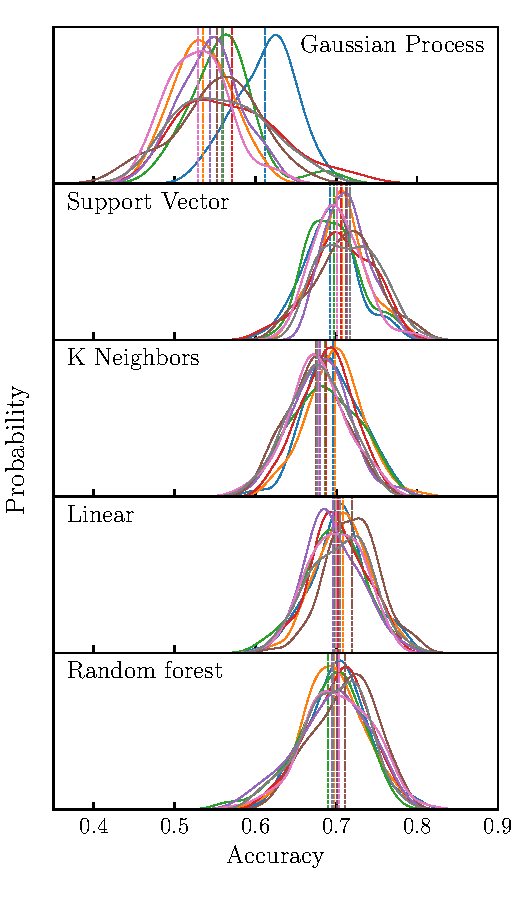
\includegraphics[width=2.8in]{figs/model_comparison.pdf}
\caption{Comparison of accuracies for each model and feature set. Different feature sets are shown in different colors, and the vertical dashed lines show the mean accuracy.}
\label{fig:accuracies}
\end{figure}

\subsection{Choosing the bracket}
When I set my bracket, I would like not only to predict the winners of each game, but to obtain for every game a probability that Team A beats Team B.
This won't affect my final bracket, of course, but it will let me see which games I ``almost got right'' and which ones I clearly got wrong.
One way to do this is to train several models (using different subsets of the training data each time) and look at every model's prediction for a given game.
If 70\% of models predict Team A to win, then Team A has a 70\% chance of winning.
Since linear regression models simply fit straight lines to the data, they very consistently pick the same winner, even if the two teams are closely matched.
Support vector regression models, while better, have a similar problem.
The random forest regressor, on the other hand, is more sensitive to the training data and is therefore more useful in making these calculations.

To make my predictions, I use the random forest regressor with Pomeroy ranking, win percentage, strength of schedule, points allowed per game, and field goal percentage as features. 
I train 250 models, using different random subsets of 10\% of all regular season data.
For each tournament game, I use all 250 models to predict the winner, and advance the team that is predicted to win by the majority of the models.
I then continue to the next round and repeat until the tournament is complete.
\href{https://fantasy.espn.com/tournament-challenge-bracket/2022/en/entry?entryID=67523739}{My final bracket is available here}, with Kentucky selected as the winner (sigh).

\subsection{How did it turn out?}
Overall, my bracket did quite well, scoring 820 points (out of 1920) and beating 89\% of all brackets submitted to ESPN.
Tragically, my pick, Kentucky, lost in the very first round in a 2-15 upset to this year's Cinderella team, Saint Peter's.
From the get-go, this lost me a total of 630 potential points.
All 250 of my models predicted Kentucky to win round 1, so this definitely wasn't an ``almost got it right'' scenario.

My models did, however, correcly predict some first-round upsets, including New Mexico State (12) vs UConn (5), Notre Dame (11) vs. Alabama (6), and Michigan (11) vs. Colorado State (6).
Most exciting, though, were the models' predictions of 8th seed North Carolina's historic run, becoming the fifth 8 seed to ever make the championship game.
Almost 90\% of the models had North Carolina (8) beating Baylor (1) in the second round.
I had them losing to Kentucky in round 4, but had I known Kentucky would lose in the first round, I might have gotten the next games right too.
Surprisingly, my K neighbors bracket had North Carolina winning the whole thing, but fared slightly worse overall, finishing in the 80th percentile.

In the end, I won all of the bracket groups I was a part of, coming out two free dinners and a six pack on top.
I consider this a resounding success.

\subsection{Future improvements}
There are certainly improvements that can be made to my model, and now that I have the framework built, it won't be as much work to implement next year:
\begin{enumerate}
\item Use more data: Due to time and resource limitations, I only used data dating back to the 2014-15 season. The available data go back much further and could provide additional insights.
\item Account for bracket scoring: The brackets are scored such that first round games are worth 10 points, second round games 20, third round games 40, and so on (${\rm points} = 10\times 2^{{\rm round}-1}$), but my algorithm treats all games equally. A model might predict a 55\% chance of a big 16-1 upset in round 1, but proceed to have the 16 seed team lose in round 2. Is it worth gambling on the upset for 10 points and risk missing out on more points from future rounds if the 1 seed team wins? Rather than pick the most likely winner for each round, one could instead optimize for the maximum expected final bracket score.
\item Account for pandemic-affected seasons: I used data from all seasons and all tournaments 2014-15 to 2021-22 to make my decisions. It might be smarter to remove the 2020-21 and 2021-22 seasons due to the effect the COVID-19 pandemic had on the games (Section \ref{sect:homecourt}). Similarly, it might not make sense to use data all the way back to 1985 since gameplay has changed since then.
\end{enumerate}


%%%%%%%%%%%%%%%%%%%%%%%%%%%%%%%%%%%%%%
%%%%%%%%%%%%%%%%%%%%%%%%%%%%%%%%%%%%%%
%%%%%%%%%%%%%%%%%%%%%%%%%%%%%%%%%%%%%%
%%%%%%%%%%%%%%%%%%%%%%%%%%%%%%%%%%%%%%


%\software{Astropy \citep{astropy:2013, astropy:2018}, Scipy \citep{scipy}}


\bibliographystyle{apj}
\bibliography{references}


\end{document}

